\documentclass[
  bibliography=totoc,     % Literatur im Inhaltsverzeichnis
  captions=tableheading,  % Tabellenüberschriften
  titlepage=firstiscover,
  fontsize=12pt, % Titelseite ist Deckblatt
]{scrartcl}

% Paket float verbessern
\usepackage{scrhack}

% Warnung, falls nochmal kompiliert werden muss
\usepackage[aux]{rerunfilecheck}

% unverzichtbare Mathe-Befehle
\usepackage{amsmath}
% viele Mathe-Symbole
\usepackage{amssymb}
% Erweiterungen für amsmath
\usepackage{mathtools}

% Fonteinstellungen
\usepackage{fontspec}
\setmainfont{Arial}
% Wenn man andere Schriftarten gesetzt hat,
% sollte man das Seiten-Layout neu berechnen lassen
\recalctypearea{}

% deutsche Spracheinstellungen
\usepackage[british]{babel}

\usepackage[
  math-style=ISO,    % ┐
  bold-style=ISO,    % │
  sans-style=italic, % │ ISO-Standard folgen
  nabla=upright,     % │
  partial=upright,   % ┘
  warnings-off={           % ┐
    mathtools-colon,       % │ unnötige Warnungen ausschalten
    mathtools-overbracket, % │
  },                       % ┘
]{unicode-math}

% traditionelle Fonts für Mathematik
\setmathfont{Latin Modern Math}
% Alternativ zum Beispiel:
% \setmathfont{Libertinus Math}

\setmathfont{XITS Math}[range={scr, bfscr}]
\setmathfont{XITS Math}[range={cal, bfcal}, StylisticSet=1]

% Zahlen und Einheiten
\usepackage[
  locale=UK,                   % deutsche Einstellungen
  separate-uncertainty=true,   % immer Unsicherheit mit \pm
  per-mode=symbol-or-fraction, % / in inline math, fraction in display math
]{siunitx}

% chemische Formeln
\usepackage[
  version=4,
  math-greek=default, % ┐ mit unicode-math zusammenarbeiten
  text-greek=default, % ┘
]{mhchem}

% richtige Anführungszeichen
\usepackage[autostyle]{csquotes}

% schöne Brüche im Text
\usepackage{xfrac}

% Standardplatzierung für Floats einstellen
\usepackage{float}
\floatplacement{figure}{htbp}
\floatplacement{table}{htbp}

% Floats innerhalb einer Section halten
\usepackage[
  section, % Floats innerhalb der Section halten
  below,   % unterhalb der Section aber auf der selben Seite ist ok
]{placeins}

% Seite drehen für breite Tabellen: landscape Umgebung
\usepackage{pdflscape}

% Captions schöner machen.
\usepackage[
  labelfont=bf,        % Tabelle x: Abbildung y: ist jetzt fett
  font=small,          % Schrift etwas kleiner als Dokument
  width=0.9\textwidth, % maximale Breite einer Caption schmaler
]{caption}
% subfigure, subtable, subref
\usepackage{subcaption}

% Grafiken können eingebunden werden
\usepackage{graphicx}

% schöne Tabellen
\usepackage{booktabs}

% Verbesserungen am Schriftbild
\usepackage{microtype}

% Literaturverzeichnis
\usepackage[
  backend=biber,
]{biblatex}
% Quellendatenbank
\addbibresource{lit.bib}
% \addbibresource{programme.bib}

% Hyperlinks im Dokument
\usepackage[
  german,
  unicode,        % Unicode in PDF-Attributen erlauben
  pdfusetitle,    % Titel, Autoren und Datum als PDF-Attribute
  pdfcreator={},  % ┐ PDF-Attribute säubern
  pdfproducer={}, % ┘
]{hyperref}
% erweiterte Bookmarks im PDF
\usepackage{bookmark}

% Trennung von Wörtern mit Strichen
\usepackage[shortcuts]{extdash}

\author{%
  Lennart Völz\\%
  \href{mailto:lennart.voelz@tu-dortmund.de}{lennart.voelz@tu-dortmund.de}%
  \and%
  Max Möller\\%
  \href{mailto:max2.moeller@tu-dortmund.de}{max2.moeller@tu-dortmund.de}%
}
\publishers{TU Dortmund – Fakultät Physik}

% Line spacing
\usepackage{setspace}
\onehalfspacing

% Margins
\usepackage[left=2.5cm, right=2.5cm, top=3.5cm, bottom=3.5cm]{geometry}

\usepackage{adjustbox}

% Allow line breaks
\sloppy


\begin{document}
%1
\maketitle
%2
\begin{frame}{\huge{Definition and motivation of problem task}}
  \begin{itemize}
    \item \textbf{Task:} Can a computer vision algorithm truthfully detect driver inattention, using a convolutional neural network? 
    \item \textbf{Motivation:} Enhancing Road Safety: Driver inattention is a leading cause of road accidents. By detecting inattention early, potential collisions and accidents can be prevented, thereby saving lives and reducing injuries.
  \end{itemize}
\end{frame}
% 
\begin{frame}{\huge{Description of the Dataset}}
  \begin{columns}
    \column{.6\textwidth}
      \begin{itemize}
        \item \textbf{Source:} \url{https://universe.roboflow.com/driver-monitoring/dmd-tfiw0} provided by Roboflow user
        \item \textbf{License:} CC BY 4.0
        \item \textbf{Content of the Dataset:} Labeled pictures in .jpg format, displaying male drivers in different states of attention
        \item \textbf{Size of the Dataset:} 14859 pictures, (train: 80 \%, valid: 13 \%, test: 7 \%)
        \item \textbf{Input features:} Greyscale image
        \item \textbf{Target:}
        \begin{itemize}
          \item[-] Dangerous driving
          \item[-] Distraction
          \item[-] Drinking
          \item[-] Safe driving
          \item[-] Sleepy driving
          \item[-] Yawn
        \end{itemize}
        \item \textbf{Prev. Work:} pretrained Roboflow interference model 
      \end{itemize}
    \column{.4\textwidth}
      \begin{figure}
        \centering
        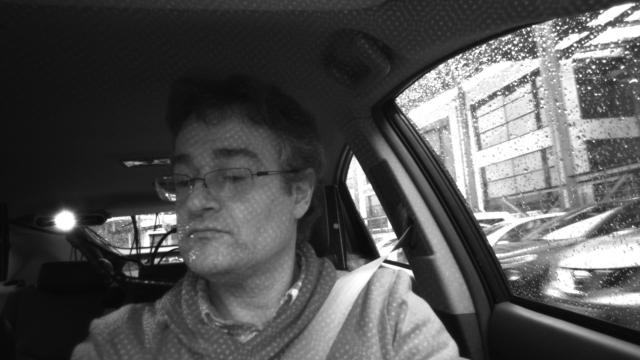
\includegraphics[width=\textwidth]{content/gA_1_s1_ir_face_mp4-26_jpg.rf.8073bccb5c613d34b8f058da71adc5d8.jpg}
        \caption{Example picture of the dataset.}
      \end{figure}
  \end{columns}
\end{frame}

\begin{frame}{\huge{Comparison to alternative methods}}
  \begin{itemize}
    \item Comparison to the pretrained model, which is accessible through the website.
    \begin{itemize}
      \item[-] Previous work is general computer vision model not specific to the dataset
      \item[-] Use precision of pretrained model as comparison baseline 
    \end{itemize}
    \vspace{5mm}
    \begin{figure}[H]
      \centering
      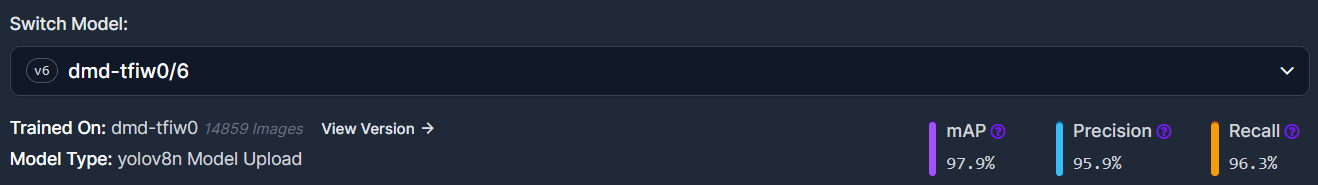
\includegraphics[width=.9\textwidth]{content/prec_pret.png}
      \caption{Precision of Roboflow interference model.}
    \end{figure}
  \end{itemize}
\end{frame}

\end{document}